\begin{center}
  \section{\capitalisewords{From Neurons to Silicon: The Neuromorphic Revolution}}
  Tiyasa Pal, 3$^{rd}$ Year, ECE
\end{center}

\setcounter{figure}{0}
\setcounter{table}{0}

\begin{multicols}{2}
  \begin{abstract}
    \bfseries
    Neuromorphic computing is an interdisciplinary hardware discipline that implements brain-inspired principles -co-located memory and computation, event-driven (spike-based) signalling, and adaptive synaptic weighting -directly in silicon, in contrast to the instruction-driven, memory-separated Von Neumann model that underlies conventional CPUs and GPUs. This report examines the architectural principles of neuromorphic systems, benchmarks representative chips quantitatively, and critically evaluates the gap between demonstrated laboratory efficiency and real-world commercial deployment.

    \noindent
    Published results indicate that the approach can deliver large efficiency gains on workloads that map naturally onto sparse, event-driven computation: IBM's NorthPole reports roughly 25× higher energy efficiency (frames-per-second per watt) than a comparable 12 nm-class GPU on the ResNet-50 image-classification benchmark, while Intel's Hala Point system (1,152 Loihi 2 chips, 1.15 billion neurons, 128 billion synapses) sustains approximately 20 petaops at over 15 trillion 8-bit operations per second per watt. Earlier devices - IBM TrueNorth (1 million neurons, 256 million synapses, 28 nm) and Intel's first-generation Loihi (131,072 neurons, 130 million synapses, 14 nm) - established the feasibility of large-scale spiking hardware but were confined to research settings.

    \noindent
    However, these efficiency figures are workload-specific rather than general-purpose: dense-matrix operations that dominate contemporary AI, such as transformer-based language models, do not map efficiently onto spiking substrates, and the absence of a mature, standardized programming model (comparable to CUDA for GPUs) remains the principal barrier to commercial adoption. This report therefore combines a technical description of neuromorphic architecture with a critical assessment of where the technology currently delivers genuine advantage, where its benefits are overstated, and what would be required for wider adoption.
  \end{abstract}

  \subsection*{\centering\uppercase{INTRODUCTION}}
  The rapid advancement of artificial intelligence and machine learning has increased the demand for faster and more efficient computing systems. Conventional computers are mainly based on the Von Neumann architecture, where memory and processing units are separated. Although this architecture has been highly successful for decades, it suffers from limitations such as high-power consumption, memory bottlenecks, and reduced efficiency in handling complex AI tasks.

  \noindent
  The human brain, by contrast, is an extremely efficient biological computing system. It contains nearly 86 billion neurons connected through trillions of synapses, enabling massive parallel processing while consuming only about 20 watts of power. Inspired by this efficiency, scientists and engineers developed the concept of neuromorphic computing, which imitates the neural structure and operation of the brain to build intelligent machines capable of learning, adaptation, and decision-making.

  \noindent
  Neuromorphic chips are specifically designed hardware systems that mimic biological neural networks. These chips use artificial neurons and synapses to process information through spikes, similar to the way neurons communicate in the human brain. Unlike traditional processors that perform sequential computation, neuromorphic chips support parallel and event-driven processing, making them well suited to specific classes of AI workloads. Today, neuromorphic computing is explored in robotics, autonomous vehicles, healthcare, cybersecurity, and edge devices, although - as this report will show- the technology remains largely confined to research and specialised deployments rather than mainstream commercial computing.

  \subsection*{\uppercase{Core Concept and Analysis}}
  \subsubsection*{Biological Inspiration: Structure of the Human Brain}
  The foundation of neuromorphic computing lies in neuroscience. The human brain is a massively parallel and energy-efficient processing system.

  \begin{enumerate}
    \item \textbf{Neurons:} Neurons are the fundamental units of the brain. Each neuron receives signals from other neurons through dendrites, processes the information in the cell body (soma), and transmits output through the axon.
    \item \textbf{Synapses:} Synapses are the connection points between neurons. They determine the strength of communication between neurons. Learning in the brain occurs through changes in synaptic strength.
    \item \textbf{Action Potentials (Spikes):} Neurons communicate using electrical impulses called spikes or action potentials. A neuron fires only when its membrane potential exceeds a certain threshold.
    \item Key Characteristics of the Brain:
      \begin{itemize}
        \item Massive parallel processing
        \item Event-driven computation (neurons activate only when needed)
        \item Adaptive learning through synaptic plasticity
        \item Fault tolerance (the brain continues functioning even with damaged neurons)
        \item Extremely low energy consumption
      \end{itemize}
  \end{enumerate}
  These characteristics form the conceptual blueprint for neuromorphic systems.

  \begin{center}
\vspace{-0.5em}
\begin{minipage}{0.98\columnwidth}
\centering
    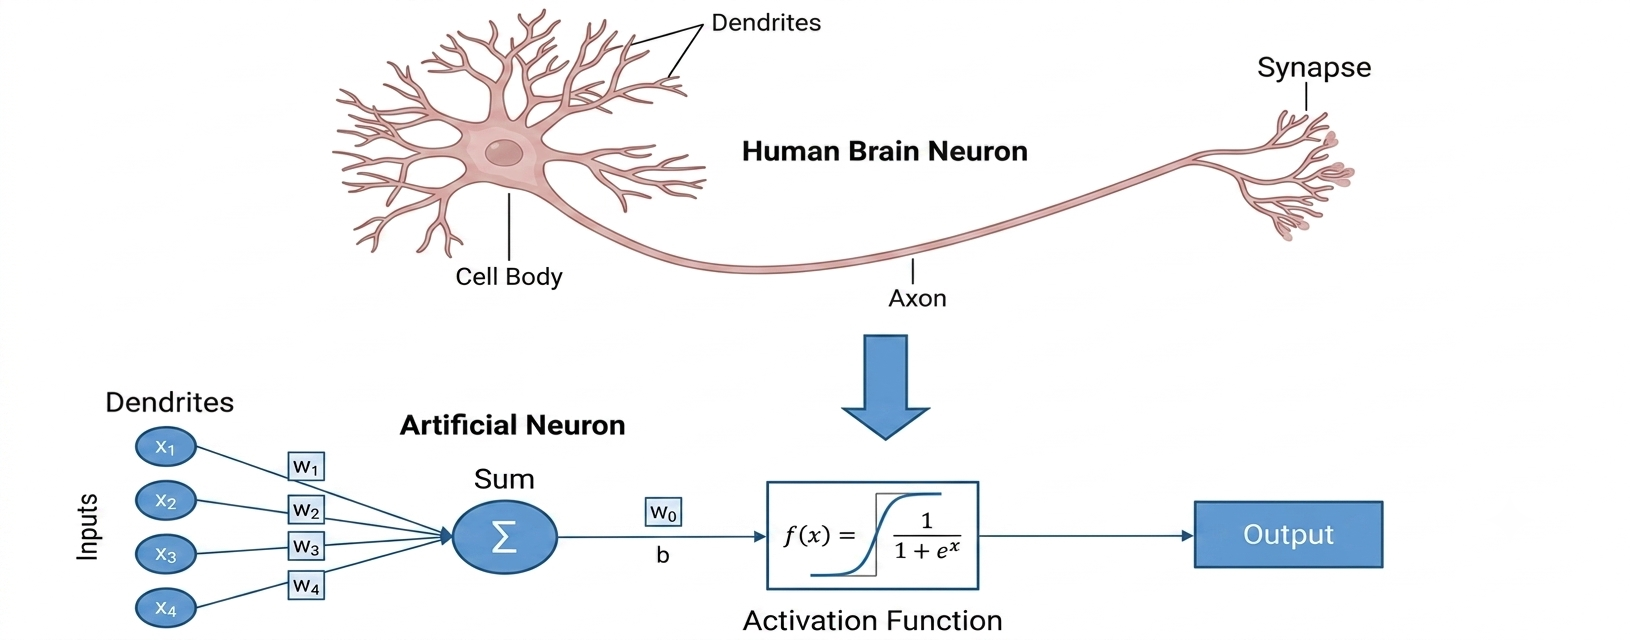
\includegraphics[width=0.85\columnwidth]{assets/images/neuron.png}
    \captionof{figure}{Schematic comparison of a biological neuron and an artificial neuron (dendrites, soma, axon, and synapse mapped to inputs, weighted sum, activation function, and output). Diagram prepared by the author to illustrate the structural analogy described by Mead [1] and Maass [2].}
\end{minipage}
  \end{center}
\vspace{-0.35em}

  \subsubsection*{Evolution from Von Neumann Architecture to Neuromorphic Design}
  Traditional computing systems follow the Von Neumann architecture, in which the CPU performs computation, memory stores data separately, and data transfer between the two creates bottlenecks — the well-known “Von Neumann bottleneck.” Neuromorphic architecture addresses this by integrating memory and computation within the same processing units, similar to synapses in the brain.

  Table~1 compares Von Neumann and neuromorphic systems.

\begin{center}
\vspace{-0.5em}
\begin{minipage}{0.98\columnwidth}
\centering
    \captionof{table}{Comparison between Von Neumann and Neuromorphic systems (adapted from principles discussed in Indiveri \& Liu [3]).}
    \setlength{\tabcolsep}{3pt}
    \renewcommand{\arraystretch}{1.3}
    \begin{tabular}{@{}>{\RaggedRight\arraybackslash}p{0.25\columnwidth}
        >{\RaggedRight\arraybackslash}p{0.26\columnwidth}
      >{\RaggedRight\arraybackslash}p{0.37\columnwidth}@{}}
      \toprule
      \textbf{Feature} & \textbf{Von Neumann Systems} & \textbf{Neuromorphic Systems} \\
      \midrule
      Processing  & Sequential & Parallel \\
      Memory      & Separate & Integrated \\
      Power Usage & High & Very Low \\
      Operation   & Clock-driven & Event-driven \\
      \bottomrule
    \end{tabular}
\end{minipage}
  \end{center}

  \begin{center}
\vspace{-0.5em}
\begin{minipage}{0.98\columnwidth}
\centering
    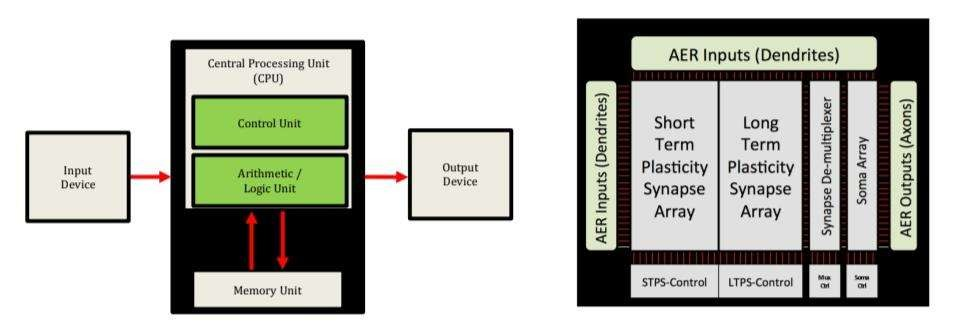
\includegraphics[width=0.85\columnwidth]{assets/images/Von Neuman system.jpg}
    \captionof{figure}{Block-level comparison of a conventional Von Neumann CPU (separated control unit, ALU, and memory) with a neuromorphic core (integrated plasticity, synapse array, and soma array addressed via AER). Diagram prepared by the author, conceptually based on Indiveri \& Liu [3] and Davies et al. [6].}
\end{minipage}
  \end{center}
\vspace{-0.35em}

  \subsubsection*{Spiking Neural Networks (SNNs)}
  Spiking Neural Networks are the computational foundation of neuromorphic systems. Unlike traditional artificial neural networks, SNNs transmit information using discrete spikes only when a neuron's membrane potential reaches a threshold, following the formulation introduced by Maass [2].

  \noindent
  Advantages of SNNs:
  \begin{itemize}\justifying
    \item Low power consumption
    \item Real-time processing capability
    \item Event-based (rather than clock-based) learning
    \item Closer biological plausibility than rate-based artificial neural networks
  \end{itemize}

  \begin{center}
\vspace{-0.5em}
\begin{minipage}{0.98\columnwidth}
\centering
    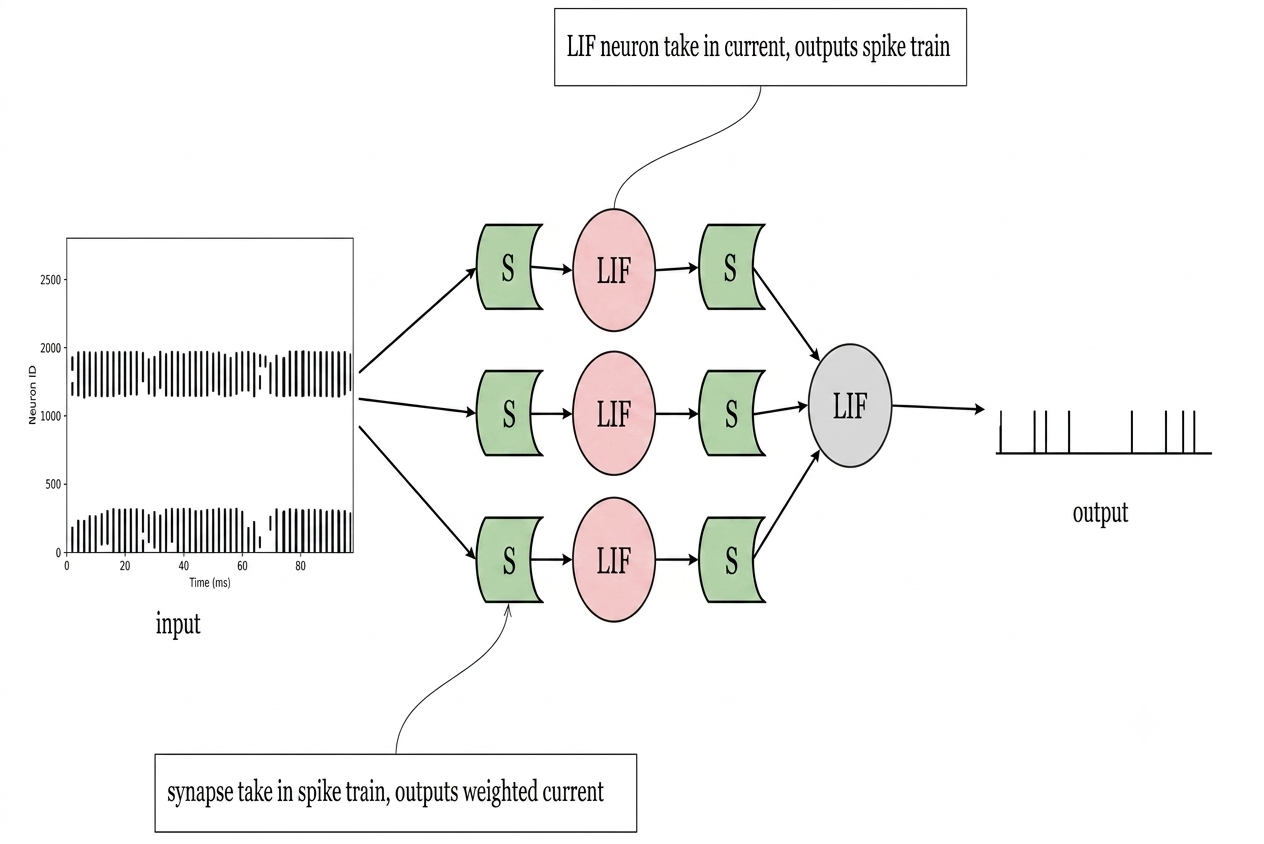
\includegraphics[width=0.85\columnwidth]{assets/images/NN.png}
    \captionof{figure}{Spiking Neural Network data flow: parallel spike-train inputs are weighted by synapse blocks (S), integrated by Leaky Integrate-and-Fire (LIF) neurons, and combined into a sparse output spike train. Diagram prepared by the author, illustrating the LIF formulation described by Maass [2] and Roy et al. [4].}
\end{minipage}
  \end{center}
\vspace{-0.35em}

  \subsubsection*{Neuromorphic Computing Architecture}
  Neuromorphic computing architecture is a brain-inspired system design that replicates the structure, functionality, and communication methods of biological neural networks. Unlike conventional computing systems that rely on a strict separation between memory and processing units, neuromorphic architecture integrates both functions into a unified framework, allowing computation to occur in a more natural, efficient, and parallel manner.
  \begin{enumerate}\justifying
    \item \textbf{Core Design Principle}
      \begin{itemize}
        \item \textbf{Eliminates bottlenecks:} traditional systems separate the CPU and memory, causing data-movement delays.
        \item Integrated units: combines processing (neurons) and memory (synapses) into a single framework.
        \item \textbf{High efficiency:} reduces data movement, improving speed and lowering power use — the same principle exploited by IBM NorthPole [12].
      \end{itemize}
    \item \textbf{Event-Driven Processing}
      \begin{itemize}
        \item \textbf{Spike-activated:} systems process data only when triggered by meaningful events (spikes).
        \item \textbf{Idle by default:} chips remain largely inactive until input signals cross a specific threshold.
        \item \textbf{Key benefit:} saves energy and enables real-time responsiveness, though only for sparse, temporally structured inputs.
      \end{itemize}

    \item \textbf{Parallel Structure}
      \begin{itemize}
        \item \textbf{Massively concurrent:} large numbers of artificial neurons compute simultaneously instead of sequentially.
        \item \textbf{Decentralised control:} processing is distributed locally across multiple independent cores.
        \item \textbf{Key benefit:} low latency and efficient scaling for workloads that are naturally distributable.
      \end{itemize}
    \item \textbf{Key Components}
      \begin{enumerate}[label=(\alph*)]
        \item \textbf{Artificial Neurons} — receive input spikes, integrate information over time, and fire an output spike when a threshold is reached, mimicking biological neuron behaviour.
        \item \textbf{Synaptic Connections} — weighted links between neurons that determine signal strength and also serve as the system's memory, since learned information is stored in synaptic weights.
        \item \textbf{Communication Networks} — neuromorphic systems use asynchronous, spike-based communication such as Address Event Representation (AER) and event-driven routing, so that only active neurons communicate.
        \item \textbf{Learning Circuits (Plasticity Mechanisms)} — adapt synaptic strengths over time using rules such as Spike-Timing-Dependent Plasticity (STDP) and Hebbian learning, enabling on-chip learning without an external training system.
      \end{enumerate}
  \end{enumerate}

  \begin{center}
\vspace{-0.5em}
\begin{minipage}{0.98\columnwidth}
\centering
    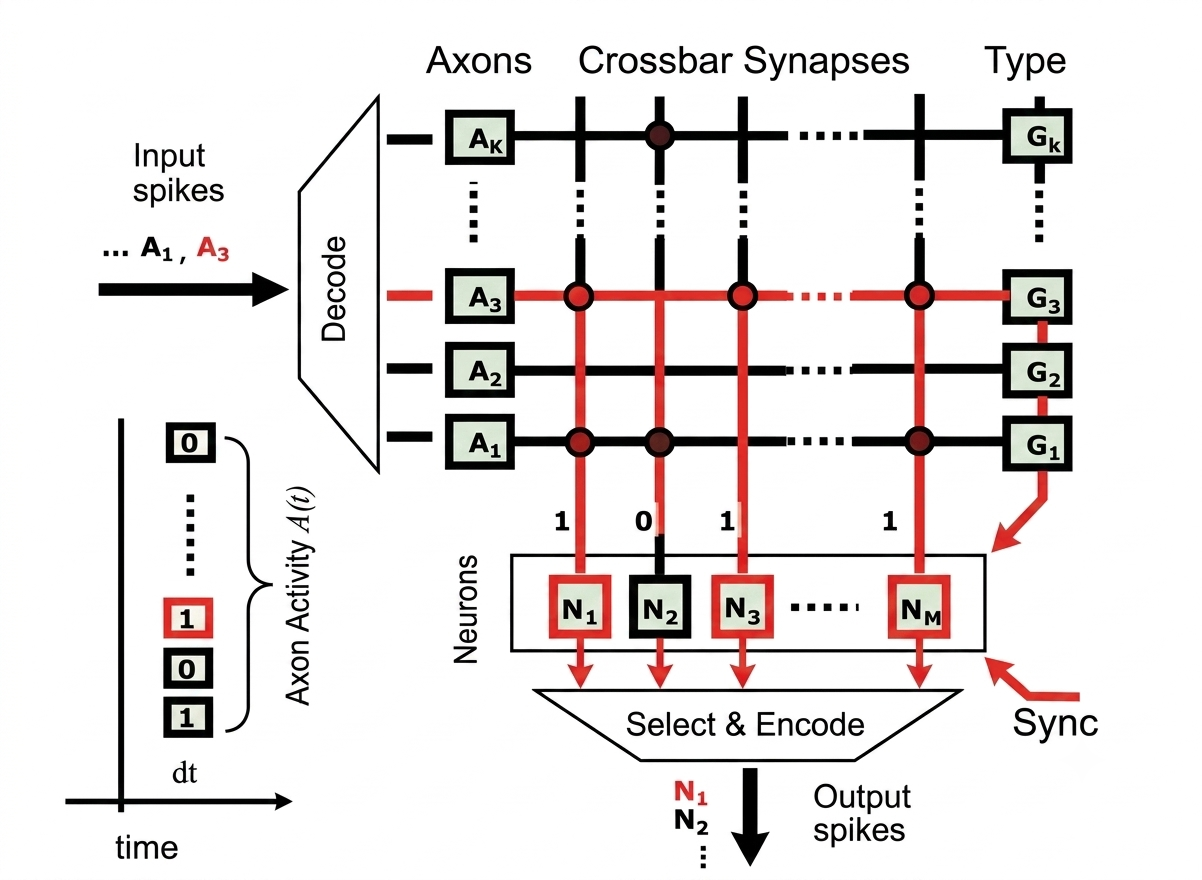
\includegraphics[width=0.72\columnwidth]{assets/images/NMC.png}
    \captionof{figure}{Simplified neuromorphic crossbar architecture: input spikes are decoded onto axons, weighted at crossbar synapse junctions, integrated by neurons $N_1$--$N_n$, and re-encoded into output spikes. Diagram prepared by the author, conceptually based on the crossbar-array designs surveyed by Schuman et al. [9].}
\end{minipage}
  \end{center}
\vspace{-0.35em}

  \subsubsection*{Major Neuromorphic Chips — Established Systems}
  \begin{enumerate}
    \item \textbf{Intel Loihi:} Intel's first-generation Loihi chip (2018) implements 131,072 neurons and 130 million synapses on a 14 nm process, using asynchronous spiking neural networks with on-chip STDP-based learning [6]. Loihi has been used mainly in robotics and academic research rather than commercial products.
    \item \textbf{IBM TrueNorth:} IBM's TrueNorth (2014) was one of the earliest large-scale neuromorphic processors, implementing 1 million neurons and 256 million synapses on a 28 nm process at roughly 65 mW per chip [5]. TrueNorth demonstrated the feasibility of implementing million-neuron systems in hardware, though, like Loihi, it saw limited commercial uptake.
    \item \textbf{SpiNNaker:} The SpiNNaker project, developed at the University of Manchester, uses massively parallel ARM-core clusters for real-time neural simulation. It is primarily used for large-scale simulation of biological brain models rather than deployed AI inference [8].
    \item \textbf{BrainScaleS:} BrainScaleS is a European neuromorphic platform that uses analog (rather than digital) neural computation to achieve very high-speed, accelerated brain simulation, trading digital precision for analog speed and energy efficiency [10].
  \end{enumerate}
  \subsubsection*{Recent Developments (2021–2026)}
  The years since the systems above were introduced have seen two significant developments that move neuromorphic computing closer to practical relevance, alongside continued evidence that broad commercial adoption remains distant.
  \begin{itemize}\justifying
    \item \textbf{Intel Loihi 2 and Hala Point:} Intel's second-generation Loihi 2 (2021) improved processing speed roughly tenfold over the original Loihi while supporting more flexible neuron models. In 2024 Intel assembled 1,152 Loihi 2 chips into Hala Point, a research-scale system with 1.15 billion neurons and 128 billion synapses, sustaining approximately 20 petaops at over 15 trillion 8-bit operations per second per watt — the largest neuromorphic system built to date [11].
    \item \textbf{IBM NorthPole:} IBM's NorthPole (2023), described by Modha et al. in Science, is not a spiking chip but a brain-inspired inference accelerator that eliminates off-chip memory access by co-locating compute and memory across its cores. On the ResNet-50 image-classification benchmark, NorthPole reports roughly 25× higher energy efficiency (frames per second per watt) and 5× higher space efficiency than a comparable 12 nm-class GPU [12]. Because NorthPole targets inference only and does not use spikes, its inclusion illustrates that “brain-inspired” efficiency gains can be achieved through memory-compute co-location alone, independent of spiking dynamics.
    \item \textbf{Edge-Oriented Commercial Chips:} Alongside these large research systems, edge-focused neuromorphic chips such as BrainChip's Akida and Innatera's mixed-signal T1 have reached commercial, milliwatt-class deployment in cameras, sensors, and wearables — a narrower but more immediately commercial application than the large research systems above.
  \end{itemize}

  \subsubsection*{Quantitative Comparison of Neuromorphic Systems}
  The table below consolidates the quantitative specifications discussed above to allow direct comparison across generations and design philosophies.
\end{multicols}
\begin{table}[tb]
\centering
\caption{Quantitative comparison of representative neuromorphic and brain-inspired computing systems.}
\small
  \setlength{\tabcolsep}{3pt}
  \renewcommand{\arraystretch}{1.2}
  \begin{tabular}{@{}>{\RaggedRight\arraybackslash}p{0.18\textwidth}
      >{\RaggedRight\arraybackslash}p{0.11\textwidth}
      >{\RaggedRight\arraybackslash}p{0.12\textwidth}
      >{\RaggedRight\arraybackslash}p{0.10\textwidth}
      >{\RaggedRight\arraybackslash}p{0.20\textwidth}
    >{\RaggedRight\arraybackslash}p{0.21\textwidth}@{}}
    \toprule
    \textbf{Chip / System} & \textbf{Neurons} & \textbf{Synapses} & \textbf{Process Node} & \textbf{Power / Efficiency} & \textbf{Status / Notes} \\
    \midrule
    IBM TrueNorth (2014) & 1 million & 256 million & 28 nm & $\sim$65 mW/chip & Early large-scale proof of concept [5] \\
    Intel Loihi (2018) & 131,072 & 130 million & 14 nm & Sub-100 mW typical & Research/robotics use [6] \\
    Intel Loihi 2 (2021) & Up to 1 million/chip & 120 million/chip & Intel 4 (7 nm-class) & $\sim$10$\times$ faster than Loihi 1 & Basis for Hala Point [11] \\
    Intel Hala Point (2024) & 1.15 billion (system) & 128 billion (system) & Intel 4 & 20 petaops; $>$15 TOPS/W & 1,152 Loihi 2 chips; research-scale [11] \\
    IBM NorthPole (2023) & 224M-parameter-class arrays & N/A (dense on-chip weights) & 12 nm & 25$\times$ FPS/W vs. comparable 12 nm GPU on ResNet-50 & Not spike-based; inference-only ASIC [12] \\
    \bottomrule
  \end{tabular}
\end{table}
\vspace{-0.18em}

\begin{multicols}{2}
  Table~2 (above) quantifies representative neuromorphic and brain-inspired systems.

  \subsubsection*{Working Principle of Neuromorphic Chips}
  Neuromorphic chips process information through interconnected artificial neurons. When a neuron receives sufficient input signals, it generates a spike that propagates to connected neurons. The operation can be summarised as follows: (1) sensory data is received as electrical signals; (2) artificial neurons integrate the signals; (3) spikes are transmitted across synapses; (4) synaptic weights are updated during learning; (5) output decisions are generated. This process closely resembles biological neural communication, though the precision with which it is implemented varies considerably across the chips discussed in Sections 3.5–3.6.

  \subsubsection*{Advantages of Neuromorphic Computing}
  \begin{enumerate}
    \item \textbf{Energy Efficiency:} Neuromorphic systems can consume significantly less power than traditional processors on workloads that suit event-driven computation, making them attractive for battery-powered devices and edge computing.
    \item \textbf{Real-Time Processing:} Parallel, event-driven architecture allows rapid processing for real-time decision-making in autonomous systems and robotics.
    \item \textbf{Scalability:} Architectures such as Loihi 2 and Hala Point demonstrate that neuromorphic systems can scale to billions of neurons and synapses, at least at the research-system level [11].
    \item \textbf{Adaptive Learning:} On-chip plasticity mechanisms such as STDP allow neuromorphic chips to adapt dynamically to environmental changes without complete retraining.
    \item \textbf{Fault Tolerance:} The distributed nature of neural systems allows neuromorphic chips to continue functioning even if some components fail.
  \end{enumerate}

  \subsubsection*{Applications of Neuromorphic Computing}
  \begin{enumerate}\justifying
    \item \textbf{Robotics:} Neuromorphic chips enable robots to process sensory information and react quickly to changing environments, supporting navigation and object recognition.
    \item \textbf{Autonomous Vehicles:} Self-driving cars require rapid decision-making based on sensor data; neuromorphic processors can improve efficiency in object detection, collision avoidance, and navigation.
    \item \textbf{Healthcare:} Applications include brain–machine interfaces, prosthetic devices, medical diagnosis, and neural monitoring systems.
    \item \textbf{Edge Computing:} Edge devices such as smartphones, IoT sensors, and drones benefit from low-power neuromorphic processing, and are, in practice, the segment where commercial deployment (Akida, Innatera T1) is furthest along.
    \item \textbf{Cybersecurity:} Neuromorphic systems can detect abnormal patterns and cyber threats in real time using adaptive learning mechanisms.
    \item \textbf{Speech and Image Recognition:} Neuromorphic processors can recognise speech patterns, facial expressions, and visual objects with reduced energy consumption relative to GPU-based pipelines, on the specific benchmark tasks reported in the literature.
  \end{enumerate}

  \subsubsection*{Critical Analysis and Challenges}
  While Sections 3.5–3.10 describe genuine engineering achievements, a critical reading of the neuromorphic computing literature reveals that the field has been described as “five years away” from commercial relevance for approximately fifteen years, and several structural issues explain why.
  \begin{enumerate}\justifying
    \item \textbf{Workload Mismatch:} The energy-efficiency figures reported for Hala Point and NorthPole are workload-specific rather than general-purpose. Sparse, temporally structured, event-driven tasks — continuous auditory processing, certain optimisation problems, and some robotics control loops — map naturally onto neuromorphic hardware. Standard image classification pipelines, and especially transformer-based large language models that dominate contemporary AI workloads, rely on dense matrix multiplication and do not map efficiently onto spike-based substrates. This means the headline efficiency multipliers cannot be generalised to “AI workloads” as a whole.
    \item \textbf{Software and Programming Ecosystem Gap:} Unlike GPU computing, which matured around a single dominant programming model (CUDA), the neuromorphic field remains fragmented across at least five materially different architectures — Loihi 2, SpiNNaker2, Akida, NorthPole, and Innatera T1 — each with its own programming model and toolchain. This fragmentation, more than any hardware limitation, is the primary obstacle to porting existing AI workloads onto neuromorphic substrates.
    \item \textbf{Hardware Complexity and Programming Difficulty:} Designing chips that accurately mimic biological neural systems remains highly complex, and neuromorphic programming models differ substantially from conventional software engineering practice, raising the barrier to entry for developers.
    \item \textbf{Limited Commercial Adoption:} With the partial exception of edge-oriented chips such as Akida and Innatera T1, neither Intel nor IBM has shipped a production, general-purpose commercial neuromorphic product; current large-scale deployments remain research partnerships and government-funded systems rather than mainstream commercial infrastructure.
    \item \textbf{Lack of Standardization:} There are no universal standards for neuromorphic hardware or software design, which complicates benchmarking, cross-vendor comparison, and the kind of ecosystem effects that accelerated GPU adoption.
    \item \textbf{Scalability Challenges:} Although Hala Point demonstrates scalability to billions of neurons, this required assembling over a thousand individual chips; whether such multi-chip systems can be made cost-effective and power-efficient at data-centre scale, rather than as research demonstrations, remains an open question.
  \end{enumerate}

  \subsubsection*{Future Scope of Neuromorphic Computing}
  Neuromorphic computing is likely to retain a meaningful, if narrower than initially projected, role in future AI systems — particularly where energy constraints dominate, such as edge AI, wearables, and always-on sensing.
  Future developments that could broaden this role include:
  \begin{itemize}\justifying
    \item A unifying software framework analogous to CUDA, potentially built around open efforts such as Intel's Lava
    \item Advanced autonomous robots exploiting low-latency, event-driven sensing
    \item Energy-efficient AI hardware for edge and wearable deployment
    \item Brain-computer interfaces requiring real-time, low-power neural signal processing
    \item Hybrid architectures that combine neuromorphic front-ends with conventional accelerators for dense computation
  \end{itemize}
  As AI continues to expand into everyday life, neuromorphic systems are likely to remain a specialised complement to, rather than a wholesale replacement for, GPU- and TPU-based computing, at least over the near-to-medium term.

  \subsection*{\centering\uppercase{Conclusion}}
  Neuromorphic computing represents a genuine and well-documented engineering achievement in brain-inspired hardware design, with systems such as Intel's Hala Point and IBM's NorthPole demonstrating substantial, quantifiable efficiency gains on the specific workloads for which they were designed. At the same time, a critical assessment of the field shows that these gains are narrower in scope than early enthusiasm suggested: the mismatch between spike-based hardware and the dense-matrix workloads that dominate modern AI, combined with a fragmented and immature software ecosystem, has kept neuromorphic computing largely confined to research systems and niche edge deployments rather than mainstream commercial adoption.

  \noindent
  Continued progress in hardware scaling, exemplified by Hala Point, and in memory-compute co-location, exemplified by NorthPole, suggests the field is advancing on solid engineering grounds. Whether it achieves broad commercial relevance will likely depend less on further hardware gains and more on the emergence of a standardised programming model and a clearer identification of the workloads for which brain-inspired computation offers a decisive advantage

  \subsection*{\centering\uppercase{References}}

  \begin{enumerate}
    \item C. Mead, “Neuromorphic electronic systems,” Proceedings of the IEEE, vol. 78, no. 10, pp. 1629–1636, 1990.
    \item W. Maass, “Networks of spiking neurons: The third generation of neural network models,” Neural Networks, vol. 10, no. 9, pp. 1659–1671, 1997.
    \item G. Indiveri and S.-C. Liu, “Memory and information processing in neuromorphic systems,” Proceedings of the IEEE, vol. 103, no. 8, pp. 1379–1397, 2015.
    \item K. Roy, A. Jaiswal, and P. Panda, “Towards spike-based machine intelligence with neuromorphic computing,” Nature, vol. 575, pp. 607–617, 2019.
    \item P. A. Merolla et al., “A million spiking-neuron integrated circuit with a scalable communication network and interface,” Science, vol. 345, no. 6197, pp. 668–673, 2014.
    \item M. Davies et al., “Loihi: A neuromorphic manycore processor with on-chip learning,” IEEE Micro, vol. 38, no. 1, pp. 82–99, 2018.
    \item A. R. Young et al., “A review of spiking neuromorphic hardware communication systems,” IEEE Access, vol. 7, pp. 135606–135620, 2019.
    \item S. B. Furber et al., “The SpiNNaker project,” Proceedings of the IEEE, vol. 102, no. 5, pp. 652–665, 2014.
    \item C. D. Schuman et al., “A survey of neuromorphic computing and neural networks in hardware,” arXiv preprint arXiv:1705.06963, 2017.
    \item C. Pehle et al., “The BrainScaleS-2 accelerated neuromorphic system with hybrid plasticity,” arXiv preprint arXiv:2201.11063, 2022.
    \item Intel Corporation, “Intel Builds World’s Largest Neuromorphic System to Enable More Sustainable AI (Hala Point),” Intel Newsroom, Apr. 2024. Loihi 2 architecture details from Intel Neuromorphic Research Community technical documentation.
    \item D. S. Modha et al., “Neural inference at the frontier of energy, space, and time,” Science, vol. 382, no. 6668, pp. 329–335, 2023. DOI: 10.1126/science.adh1174.
    \item Recent review: “A New Era in Computing: A Review of Neuromorphic Computing Chip Architecture and Applications,” Chips, vol. 5, no. 1, article 3, 2026. DOI: 10.3390/chips5010003.
  \end{enumerate}
\end{multicols}
% Full-width info box outside multicols
\begin{center}
  \begin{minipage}{\textwidth}
    \begin{tcolorbox}[
  colback=yellow!7,
  colframe=blue!35!black,
  colbacktitle=yellow!75!orange,
  coltitle=blue!25!black,
  title=\MakeUppercase{Did You Know?},
  fonttitle=\large\bfseries\sffamily,
  toptitle=1.5mm,
  bottomtitle=1.5mm,
  boxrule=0.7pt,
  arc=0mm,
  left=4mm,
  right=4mm,
  top=2.5mm,
  bottom=2.5mm
]
\footnotesize
\noindent
\begin{minipage}[t]{0.48\linewidth}
  {\sffamily\bfseries\textcolor{blue!35!black}{THE 2.15 dB DIFFERENCE}}\par
  A half-wave dipole has approximately \(2.15\text{ dBi}\) gain. Therefore,
  \(0\text{ dBd}=2.15\text{ dBi}\).

  \vspace{0.18em}
  {\sffamily\bfseries\textcolor{blue!35!black}{GAIN REDIRECTS ENERGY}}\par
  Antenna gain does not create extra transmitter power; it concentrates the
  available radiation more strongly in selected directions.
\end{minipage}
\hfill
\begin{minipage}[t]{0.48\linewidth}
  {\sffamily\bfseries\textcolor{blue!35!black}{THE 3 dB RULE}}\par
  A \(3\text{ dB}\) increase represents approximately twice the power, while
  a \(3\text{ dB}\) decrease represents half the power.

  \vspace{0.18em}
  {\sffamily\bfseries\textcolor{blue!35!black}{FREQUENCY SETS THE SCALE}}\par
  Since \(\lambda=c/f\), antennas designed for higher frequencies are
  generally physically smaller than antennas designed for lower frequencies.
\end{minipage}
\end{tcolorbox}
  \end{minipage}
\end{center}